\documentclass{article}
\author{Toby {Cathcart Burn}}
\title{The Area of the Pythagoras Tree}

\usepackage{tikz}
%\usetikzlibrary{lindenmayersystems}
\usepackage{ifthen}
\usepackage{pgf}
\newcommand{\tree}[1]{
	\fill[fill=black] (0,0) -- (1,0) -- (1,1) -- (0,1) -- cycle;
	\ifthenelse{#1<2}{}{
		\begin{scope}[yshift=1cm,rotate=45,scale=0.7071]
			\tree{\the\numexpr#1-1}
		\end{scope}
		\begin{scope}[xshift=0.5cm,yshift=1.5cm,rotate=-45,scale=0.7071]
			\tree{\the\numexpr#1-1} 
		\end{scope}
}}
\begin{document}
\maketitle
\begin{abstract}
The area of the Pythagoras Tree is exactly
	
${12823413011547414368862997525616691741041579688920794331363953564934456759066858494476606822552437442098640979}\over{877512406035620068631903180662851572553488753575243048137500508983979170248733422547196905684808937723408093}$.
	
This can be shown by describing the Pythagoras Tree as non-deterministic Buchi automaton with 103 states %(28-3)*4-2+1+4
and a 4 symbol alphabet.
\end{abstract}
\section{Introduction}
The Pythagoras Tree is a fractal constructed by taking a unit square and then recursively constructing 2 copies of the Pythagoras tree each scaled by a factor of $1/\sqrt{2}$ and rotated $45^\circ$ so that the bases of the copies of the original square form a right-angled isosceles triangle with the top edge of the original square.


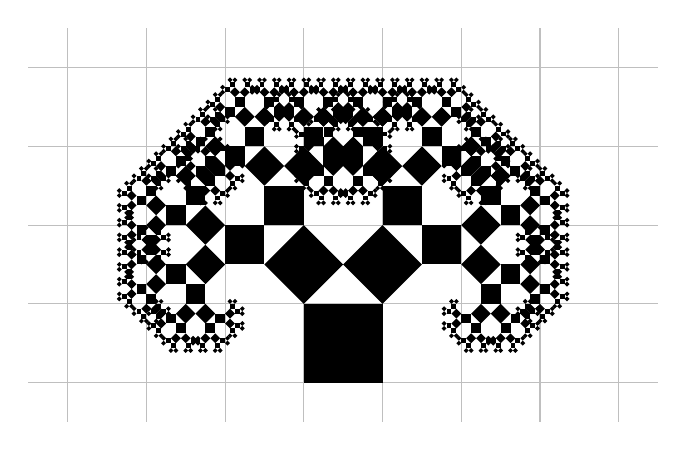
\begin{tikzpicture}[scale=1]
\draw[color=lightgray, step=1] (-3.5,-0.5) grid (4.5,4.5);

\tree{10}
\end{tikzpicture}


\end{document}
